

\begin{table}[htb]
    \renewcommand{\arraystretch}{1.5}
    \begin{tabular*}{\textwidth}{|>{\columncolor{orange!15}}p{3cm}|p{17.3cm}|}
    \textbf{\large Finding} & \textbf{\large Vulnerable Apache Version}\section*{}\addcontentsline{toc}{section}{Finding 7 - Vulnerable Apache Version}
    \\
    Risk& Medium\\
    Category& Vulnerable Software Version\\
    Impact& The client may not interpret security-related headers if a malicious backend causes the response headers to be truncated early, resulting in some headers being included in the response body. An attacker can perform HTTP Request Smuggeling due to inconsistend interpretation of HTTP Requests.
    CVE-2022-37436, CVE-2022-36760\\\\ 
    Description&
    An nmap scan illustrated the Apache version. 
    \newline
    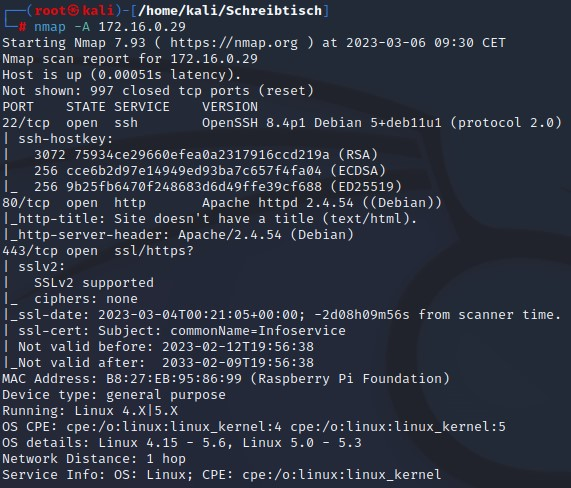
\includegraphics[width=0.73\textwidth]{vulnerable_software.jpg} 
    \newline  
    The apache version ''Apache 2.4.54'' has several vulnerabilites.
	\\ 
	&\\
	&\\
	&\\
    Recommendation& Patch your OpenSSH Version to a newer, not vulnerable version.\\    
    \\\\\\\\\\\\\\\\\\\\\\\\
    \end{tabular*}
    \end{table}